% diagrams-Bd.tex
\begin{hcarentry}[updated]{diagrams}
\report{Brent Yorgey}%05/11
\status{alpha, active development}
\participants{Ryan Yates}
\makeheader

The diagrams library provides an embedded domain-specific language for
declarative drawing.  The overall vision is for diagrams to become a
viable alternative to DSLs like MetaPost or Asymptote, but with the
advantages of being \emph{declarative}, describing what to draw, not
how to draw it, and \emph{embedded}, putting the entire power of
Haskell (and Hackage) at the service of diagram creation.

%**<img width=500 src="./paradox.jpg">
%*ignore
\begin{center}
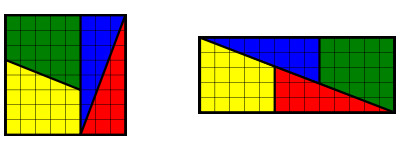
\includegraphics[width=0.47\textwidth]{html/paradox.jpg}
\end{center}
%*endignore

Since the last HCAR, the library has undergone a complete rewrite, and
now features an elegant foundational model, pluggable rendering
backends, and support for arbitrary vector spaces.

%**<img width=500 src="./triangular-numbers.jpg">
%*ignore
\begin{center}
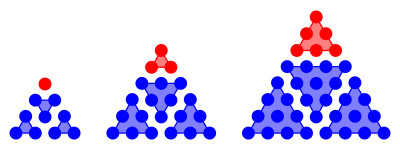
\includegraphics[width=0.47\textwidth]{html/triangular-numbers.jpg}
\end{center}
%*endignore

\FuturePlans

A preview release is imminent, with a full-featured release including
extensive documentation and tutorials planned by the end of the
summer.  Now that the core library has mostly stabilized, we hope to
attract many contributors to expand the standard library and build
higher-level drawing modules on top of the flexible core.

\FurtherReading
\url{http://code.google.com/p/diagrams}
\end{hcarentry}
